\documentclass[tikz, border=5mm]{standalone}
\usetikzlibrary{positioning, arrows.meta, calc, fit, backgrounds, shapes.geometric, patterns, decorations.pathreplacing}

\begin{document}
	
	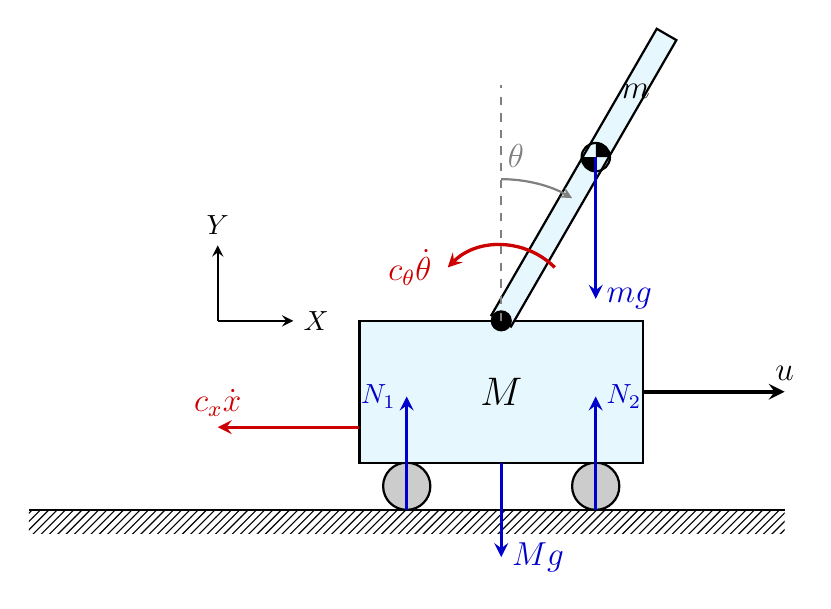
\begin{tikzpicture}[>=stealth, scale=1.2]
		
		% Definición de parámetros
		\def\W{3}         % Ancho del carro
		\def\H{1.5}       % Alto del carro
		\def\x{3}         % Posición actual x del carro
		\def\L{2}         % Longitud del péndulo al CM
		\def\Ltotal{3.5}  % Longitud física de la barra
		\def\ang{30}      % Ángulo theta en grados
		\def\Rrueda{0.25} % Radio de las ruedas
		
		% --- 1. SUELO Y REFERENCIA FIJA ---
		\draw[thick] (-2, 0) -- (6, 0);
		\fill[pattern=north east lines] (-2, -0.25) rectangle (6, 0);
		
		\draw[->, thick] (0, 2) -- (0.8, 2) node[right] {$X$};
		\draw[->, thick] (0, 2) -- (0, 2.8) node[above] {$Y$};
		
		% --- 2. EL CARRO ---
		\coordinate (CentroCarro) at (\x, \Rrueda);
		
		% Ruedas
		\draw[thick, fill=gray!40] (\x - \W/2 + 0.5, \Rrueda) circle (\Rrueda);
		\draw[thick, fill=gray!40] (\x + \W/2 - 0.5, \Rrueda) circle (\Rrueda);
		
		% Cuerpo del carro
		\draw[thick, fill=cyan!10] (\x - \W/2, 2*\Rrueda) rectangle (\x + \W/2, 2*\Rrueda + \H);
		\node at (\x, 2*\Rrueda + \H/2) {\Large $M$};
		
		% --- 3. EL PÉNDULO ---
		\coordinate (Pivote) at (\x, 2*\Rrueda + \H);
		
		% Centro de Masas (CM)
		\coordinate (CM) at ({\x + \L*sin(\ang)}, {2*\Rrueda + \H + \L*cos(\ang)});
		
		% Barra del péndulo
		\draw[thick, fill=cyan!10, rotate around={-\ang:(Pivote)}] (\x-0.12, 2*\Rrueda + \H) rectangle (\x+0.12, 2*\Rrueda + \H + \Ltotal);
		
		% Eje central del pivote
		\draw[thick, fill=black] (Pivote) circle (0.1);
		
		% Punto del Centro de Masas y etiqueta de masa m
		\begin{scope}[shift={(CM)}]
			\fill[black] (0,0) -- ++(0.15,0) arc (0:90:0.15) -- cycle;
			\fill[black] (0,0) -- ++(-0.15,0) arc (180:270:0.15) -- cycle;
			\draw[thick] (0,0) circle (0.15);
			\node[right=0.2cm] at (0,0.7) {\large $m$}; % Coherencia con figuras anteriores
		\end{scope}
		
		% --- 4. VECTORES DE FUERZA (Diagrama de Sólido Libre) ---
		
		% Acción de control u
		\draw[->, line width=1.5pt] (\x + \W/2, 2*\Rrueda + \H/2) -- ++(1.5, 0) node[above] {\large $u$};
		
		% Fuerzas de Gravedad y Normales (Azul)
		\draw[->, very thick, blue!80!black] (CM) -- ++(0, -1.5) node[right] {\large $mg$};
		\draw[->, very thick, blue!80!black] (\x, 2*\Rrueda) -- ++(0, -1) node[right] {\large $Mg$};
		\draw[->, very thick, blue!80!black] (\x - \W/2 + 0.5, 0) -- ++(0, 1.2) node[left] {$N_1$};
		\draw[->, very thick, blue!80!black] (\x + \W/2 - 0.5, 0) -- ++(0, 1.2) node[right] {$N_2$};
		
		% Fuerzas de Fricción (Rojo)
		\draw[->, very thick, red!80!black] (\x - \W/2, 2*\Rrueda + \H/4) -- ++(-1.5, 0) node[above] {\large $c_x \dot{x}$};
		
		% CORRECCIÓN: Fricción viscosa del péndulo en sentido ANTIHORARIO
		% Se cambia la dirección de la flecha (de <- a ->) y se ajustan los ángulos
		\draw[->, very thick, red!80!black] (\x, 2*\Rrueda + \H) ++(45:0.8) arc (45:135:0.8) node[left, xshift=-2pt] {\large $c_\theta \dot{\theta}$};
		
		% --- 5. INDICADORES DE MOVIMIENTO ---
		\draw[->, thick, gray] (\x, 2*\Rrueda + \H + 1.5) arc[start angle=90, end angle={90-\ang}, radius=1.5];
		\node[gray] at ({\x + 0.6*sin(\ang/2)}, {2*\Rrueda + \H + 1.5*cos(\ang/2) + 0.3}) {\large $\theta$};
		\draw[dashed, thick, gray] (Pivote) -- ++(0, \L + 0.5);
		
	\end{tikzpicture}
	
\end{document}